% ============| INÍCIO |===================
% --------------| Q01 |--------------------
\addcontentsline{toc}{section}{Questão}
\begin{prob}
  Considere a distribuição Gaussiana:
  \begin{align}
    p(x)=\frac{1}{\sqrt{2\pi\sigma^2}}\mathrm{e}^{-\frac{1}{2}\left(\frac{x-\mu}{\sigma}\right)^2}
  \end{align}
  onde $\sigma$ é o desvio padrão e $\mu$ a média. Faça plots de $p(x)$ contra $x$ para:
  \begin{enumerate}[label=\alph *)]
    \item $\mu=0$ e $\sigma=0,1$
    \item $\mu=1$ e $\sigma=0,1$
    \item $\mu=0$ e $\sigma=1$
    \item $\mu=1$ e $\sigma=1$
  \end{enumerate}
  Comente a semelhança e diferença entre os casos.
  \newpage
  \begin{sol}
  \par\noindent As \autoref{fig:gaussianas-1} e \autoref{fig:gaussianas-2}, mostram os gráficos das distribuições gaussianas $p(x)$ cada qual com médias $\mu$ e desvios padrão $\sigma$ indicado.
      \begin{figure}[!htb]
      \centering
      \subfloat[$\mu=0$ \label{fig:figura01}]{
        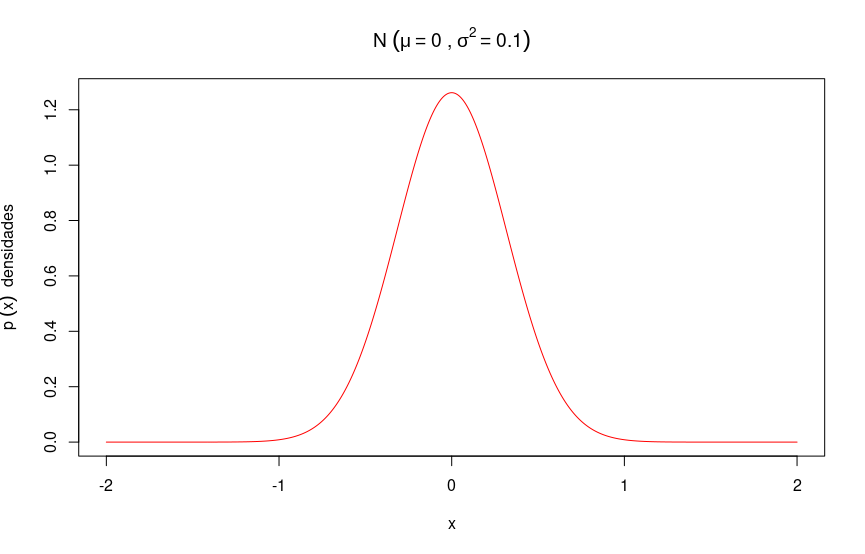
\includegraphics[width=0.48\textwidth]{img/N-m0-s01.png}
      }\hfill
      \subfloat[$\mu=1$ \label{fig:figura02}]{
        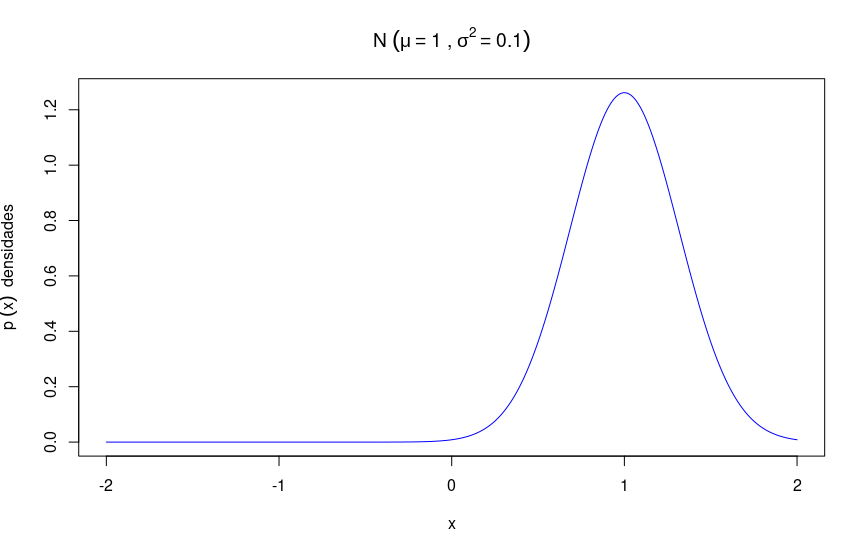
\includegraphics[width=0.48\textwidth]{img/N-mu1-s001.png}
      }        
      \caption{Distribuições gaussianas de mesma variância $\sigma^2=0,01$}
      \label{fig:gaussianas-1}       
    \end{figure}
    \begin{figure}[!htb]
      \centering
      \subfloat[$\mu=0$ \label{fig:figura03}]{
        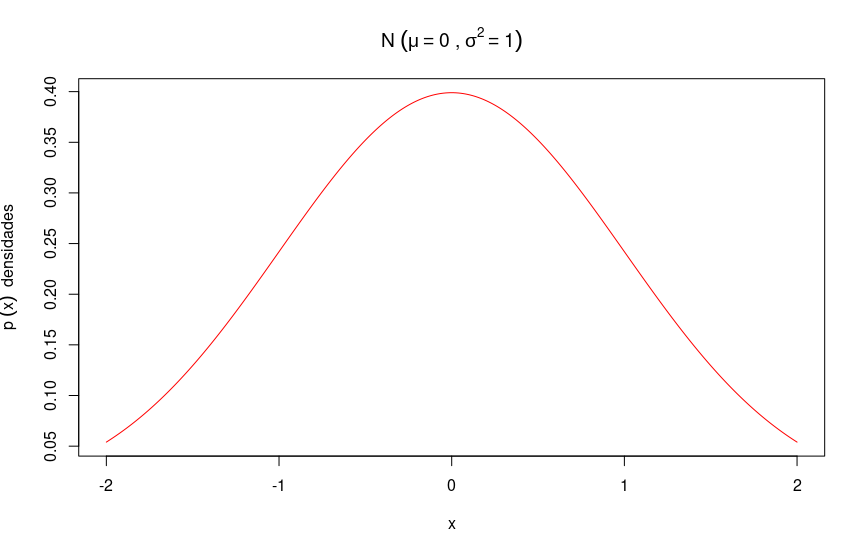
\includegraphics[width=0.48\textwidth]{img/fig-c.png}
      }\hfill
      \subfloat[$\mu=1$ \label{fig:figura04}]{
        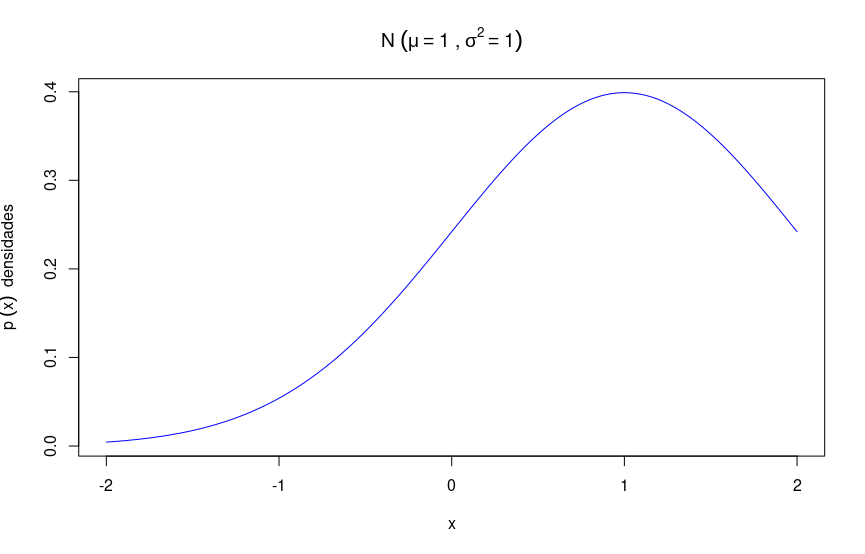
\includegraphics[width=0.48\textwidth]{img/fig-d.png}
      }        
      \caption{Distribuições gaussianas de mesma variância $\sigma^2=1$}
      \label{fig:gaussianas-2}       
    \end{figure}
    \begin{enumerate}[label=\alph *)]
      \item O gráfico da Figura\autoref{fig:figura02} assim como o gráfico da Figura\autoref{fig:figura04}, tem a sua forma deslocada para a direita, com relação aos gráficos da Figura\autoref{fig:figura01} e da Figura\autoref{fig:figura03} respectivamente, indicando que a curva é simétrica com relação a média $\mu$ e consequentemente, uma densidade de probabilidade maior em torno dessa média.
      \item Já os gráficos da \autoref{fig:gaussianas-1} diferem com relação aos gráficos da \autoref{fig:gaussianas-2}, pelo "achatamento" da curva, o que evidencia uma maior dispersão dos valores em torno da média. Quanto maior a variância $\sigma^2$, mais dispersos serão os valores da variável que se enquadra neste tipo de distribuição. 
    \end{enumerate}
  \end{sol}
\end{prob}